\newpage
\section{Viewers}
\label{sec:viewers}

\begin{description}
 %------------------------------------------------------------------------------
\addcontentsline{toc}{subsection}{btkSlicesMotionViewer}
\item[btkSlicesMotionViewer]: Construct a VTK polydata wich outline the slice for each input. Transforms can be given in output the option \texttt{-r} will open a render window.
A typical use of this program is to visualize slice by slice transformation onto volume. See figure~\ref{fig:btkSlicesMotionViewer}.

Recommended usage: \texttt{btkSlicesMotionViewer -i ana01.nii.gz $\cdots$ -i anaN.nii.gz -t transform01.txt $\cdots$ -t transformN.txt -o PolyData01.vtk $\cdots$ -o PolyDataN.vtk -r }

Note that the only required arguments are the inputs and outputs.

\begin{figure}[t]
\centering
\begin{tabular}{ccc}
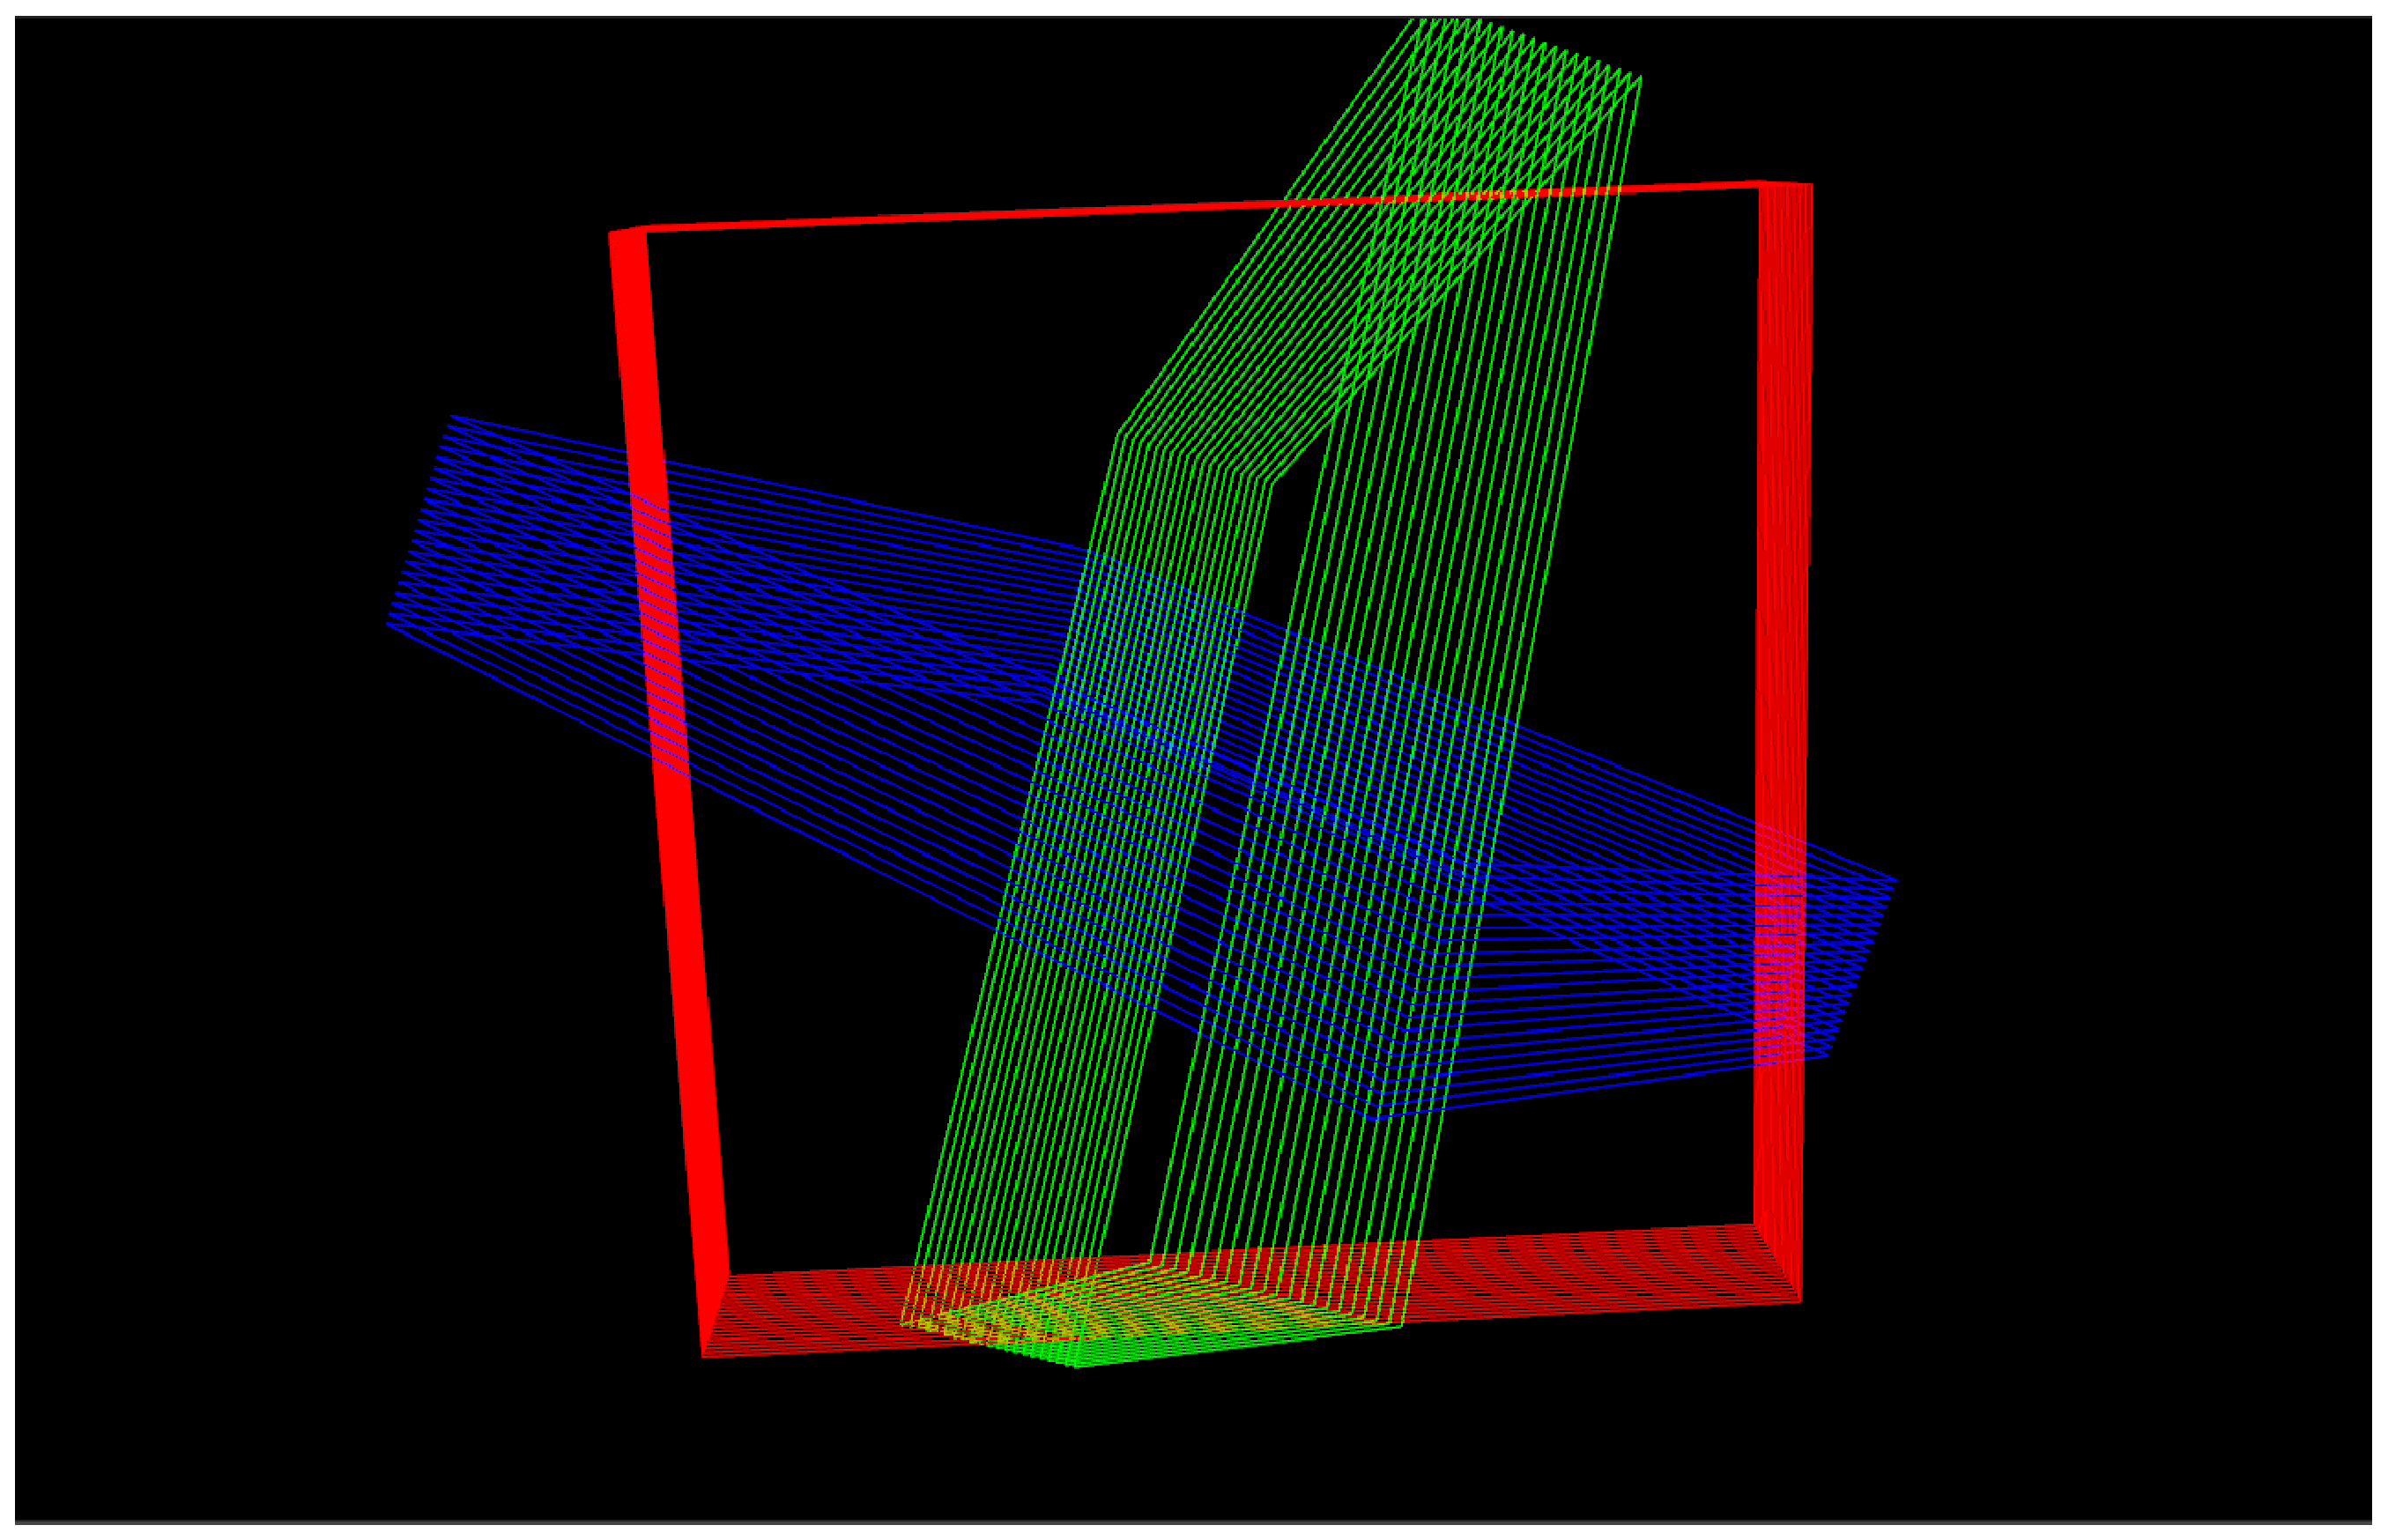
\includegraphics[width=0.5\columnwidth]{btkSlicesMotionViewer.eps}
\end{tabular}
\caption{Example of a render of three polydatas (axial, coronal, and sagital).
\texttt{btkSlicesMotionViewer}.}
\label{fig:btkSlicesMotionViewer}
\end{figure}

%------------------------------------------------------------------------------
\addcontentsline{toc}{subsection}{btkDiffusionViewer}
\item[btkDiffusionViewer]: Usefull for diffusion dataset visualization (memory consuming). The option \texttt{--percent\_of\_sample\_points} can be used to set the percent of points (of the number of voxels) being sampled for modeling display. This can be usefull for memory saving and spacing control between model representations. An other usefull option is the input mask (\texttt{-m}) used to mask a part of the image.
Once the display window is opened, you can move the slice up and down by using the corresponding arrows of your keyboard. To display the mean directions and the modeling, you can use respectively the touch 'd' and 'm' of your keyboard.
%------------------------------------------------------------------------------

\end{description}

